This chapter presents an extensive tracking performance study with the OpenDataDetector (ODD) using Acts and its Examples. Performance results are obtained for all algorithms of the tracking chain, from seeding to primary vertexing, with particular focus on track finding and fitting. The performance is evaluated using various metrics, including efficiency, fake rate, and resolutions and pulls of estimated track and vertex parameters. The results are presented for different single particle samples ($\mu$, $\pi$, $e$) and for \ttbar events with different pileup scenarios. Reconstructed quantities are compared to the truth information to assess the quality of the reconstruction.

A subset of this study has already been presented at the 2023 Connecting the Dots (CTD) conference \cite{ctd-acts-odd}. Due to previous limitations of the track finding algorithm, the CTD study only considered truth-based track seeding. This gap is filled here by including the performance of the triplet seeding algorithm and the improved version of the track finding algorithm.

The chapter is structured as follows: first, the simulation setup is described and the generated samples are layed out. Then, the reconstruction chain is presented. Followed by the performance of the seeding, track finding, ambiguity resolution, track refitting, and primary vertexing. Finally, the computation time of the reconstruction chain is discussed.

\section{Event generation and simulation}

Acts Examples offer different methods for event generation, simulation, and digitization. Event generation can be done with a particle gun or with Pythia8 \cite{pythia8}. In this study, a particle gun is used to generate single $\mu$, $\pi$, and $e$ to estimate the reconstruction performance under ideal conditions. Pythia8 is used to generate \ttbar events with different pileup scenarios, which are more realistic and closer to the conditions in a real hadron collider experiment. Both event simulators, Fatras (see Section \ref{sec:intro/acts/fatras}) and Geant4 \cite{geant4-2003}\cite{geant4-2006}\cite{geant4-2016}, are used to simulate the passage of the generated particles through the detector. This allows to cross-check the reconstruction results and can help to identify potential issues in the simulation or reconstruction chain. For instance, Fatras uses the same material model as the reconstruction, which provides optimal conditions in terms of material handling.

Simulated hits coresponding to energy deposits in sensitive detectors undergo a digitization process to mimic the behavior of detector electronics and to produce read out signals.

The OpenDataDetector does not provide a realistic digitization, but Acts Examples offers two fast, truth-based digitization methods: smeared digitization and geometric digitization. The smeared digitization converts simulated hits into measurements by applying user-provided noise. The true measurement uncertainty is passed to the reconstruction. The geometric digitization uses sensor segmentation to estimate activation of cells, based on the path of the particle. These cells are directly turned into measurements. For this study, the smeared digitization is used to create measurements from the simulated hits, as the geometric digitization is not fully validated yet.

The OpenDataDetector is used as a detector in optimal conditions: perfect alignment, perfect knowledge about material amount and placement, and perfect knowledge about the magnetic field.

The following events have been simulated and form the basis for the performance study:
\begin{itemize}
    \item 100k single $\mu$, $\pi$, $e$ for each $p_T \in \{1,10,100\}$ GeV, with random charge, uniform $\eta \in [-3,3]$, and uniform $\phi$, generated with a particle gun
    \item 100k single $\mu$, $\pi$, $e$ with exponentially distributed $p_T \in [1,100]$ GeV, random charge, uniform $\eta \in [-3,3]$, and uniform $\phi$, generated with a particle gun
    \item 1k \ttbar events with 200 pileup interactions, generated with Pythia8
    \item using Fatras and Geant4 for event simulation
    \item using smeared digitization
\end{itemize}

Particles and hits are stored in ROOT \cite{root} files and are later consumed by the reconstruction chain as inputs. This allows to switch the digitization method without running the event simulation again.

\section{Reconstruction chain and cuts}

The event reconstruction is implemented on top of the existing components in Acts Examples. The reconstruction chain consists of the following steps: Truth-based measurement formation, spacepoint creation, seeding, track finding, ambiguity resolution, track refitting, and primary vertexing. The individual steps and their performance are described in the following sections. It should be noted that the simulation and reconstruction use the same magnetic field, material, and alignment conditions.

Acts Examples provides different truth based algorithms for track seeding, track finding, vertex seeding, and vertex finding. These algorithms allow to evaluate the performance of individual algorithms under ideal conditions. Truth-based algorithms were used during this study to compare the performance of the reconstruction chain with and without truth information.

Since the ODD provides time information in the pixel system, the reconstruction chain was designed to support 4D reconstruction as much as possible (see Chapter \ref{ch:dev/4d_tracking}). This includes spacepoint creation, parameter estimation, track finding, track fitting, vertex finding, and vertex fitting.

Before measuring the performance of the reconstruction chain, a choice of cuts is made to select the particles and measurements that are used for the performance evaluation. The following truth cuts are applied to the simulated particles:

\begin{itemize}
    \item true $p_T \ge 1 \text{GeV}$
    \item true $|\eta| < 3.0$
    \item true $q \ne 0$
    \item measurements $\ge 6$
    \item measurements in pixels $\ge 3$
\end{itemize}

Similarly, cuts are applied during reconstruction to isolate objects of interest. The following cuts are applied to reconstructed tracks:

\begin{itemize}
    \item reconstructed $p_T > 0.7 \text{GeV}$
    \item reconstructed $|\eta| < 3.5$
    \item measurements on track $\ge 6$
    \item outliers and/or holes on track $\le 3$
\end{itemize}

After objects have been reconstructed, truth information is used to match the reconstructed objects to the truth particles. This allows to evaluate the performance of the reconstruction algorithms. The following cuts are applied to match reconstructed objects to truth:

\begin{itemize}
    \item \textbf{seed:} 100\% of the measurements forming a seed must be matched to the same truth particle
    \item \textbf{track:} 50\% of the measurements forming a track must be matched to the same truth particle \textbf{and} 50\% of the measurements of the truth particle must be covered by the track (called \textit{double matching})
    \item \textbf{vertex:} 70\% of the track weight must be matched to truth particles coming from the same interaction
\end{itemize}

Tracks can be shared between multiple reconstructed vertices. Track weight is a measure of how well a track matches to a vertex, relative to the other vertices. A vertex with 70\% correctly assigned track weight is considered as reconstructed \textit{cleanly}.

\begin{figure}[h!]
    \centering
    
\includegraphics[width=1.0\textwidth]{parts/3_performance/11_odd-performance/figures/detector_efficiency_mixed.pdf}
    \caption{Detector efficiency, without reconstruction, as a function of $\eta$ for single $\mu$, $\pi$, and $e$ with $p_T = 10$ GeV.}
    \label{fig:perf/odd/detector-efficiency-mixed}
\end{figure}

An upper bound for the physics efficiency can be estimated using the truth cuts applied after simulation without reconstruction. The efficiency is defined as the ratio of particles that meet the truth cuts to the number of generated particles. Figure \ref{fig:perf/odd/detector-efficiency-mixed} shows the optimal physics efficiency for single $\mu$, $\pi$, and $e$ with $p_T$ = 10 GeV as a function of $\eta$. The observed efficiency is above 99\% and similar for $\mu$ and $e$, but generally lower for $\pi$. This is due to hadronic interactions of the $\pi$ with the material, before the hit criteria is met.

Efficiencies shown in the following sections are defined as the ratio of reconstructed particles with at least one matched object to the number of particles that meet the truth cuts. This is called \textit{technical efficiency} and is used to evaluate the performance of reconstruction algorithms. The technical efficiency is not a direct measure of the physics efficiency since it does not take all generated particles into account. Given the measurement requirements, this definition of efficiency does not account for sensor inefficiencies and inelastic material interactions in the detector.

\begin{figure}[h!]
    \centering
    
\includegraphics[width=1.0\textwidth]{parts/3_performance/11_odd-performance/figures/detector_material.pdf}
    \caption{Material validation up to the long strip system for $X/X_0$ as a function of $\eta$ between Acts and Geant4.}
    \label{fig:perf/odd/detector-material}
\end{figure}

Figure \ref{fig:perf/odd/detector-material} shows the material validation up to the long strip system for $X/X_0$ as a function of $\eta$ between Acts and Geant4. The observed material in Acts is within 10\% in agreement to Geant4 for most of the $\eta$ range. There are some discrepancies at $|\eta| \approx 0.3$ and $|\eta| \approx 1.0$. These bigger differences may be due to Geant4 steps that already reach into the solenoid.

\section{Seeding performance}

Seeding is the first step towards finding tracks after spacepoint creations. Acts Examples offers different seeding algorithms, including truth-based seeding and triplet seeding. Truth-based seeders can be used to evaluate the performance of the reconstruction chain under optimal conditions. The triplet seeding is a more realistic approach and can be used in real experiments. The core idea of the triplet seeding algorithm is to process all possible combinatorics of three spacepoint and select the ones that may have been produced by a single particle.

It should be noted that the triplet seeding algorithm and its configuration are currently not optimized for the ODD. Due to that reason it may produce low efficiency and high fake rates. Achieving optimal performance with the triplet seeding algorithm was not an objective of this study.

\begin{figure}[h!]
    \centering
    
\includegraphics[width=1.0\textwidth]{parts/3_performance/11_odd-performance/figures/seeding_efficiency_mu.pdf}
    \caption{Technical seeding efficiency as a function of true $\eta$ for single $\mu$ with $p_T = 1,10,100$ GeV.}
    \label{fig:perf/odd/seeding-efficiency-mu}
\end{figure}

Figure \ref{fig:perf/odd/seeding-efficiency-mu} shows the seeding efficiency for single $\mu$ as a function of true $\eta$ for different $p_T$ values. The technical efficiency is defined as the ratio of reconstructed particles with at least one matched seed to the number of selected particles, passing the hit requirement. The matching requires all three spacepoints to come from the same truth particle. The observed efficiency is high for all three $p_T$ values. There are inefficiencies at $|\eta| \approx 2$, which is likely due to suboptimal seeding configuration.

\begin{figure}[h!]
    \centering
    
\includegraphics[width=1.0\textwidth]{parts/3_performance/11_odd-performance/figures/seeding_redundancy.pdf}
    \caption{Average seed redundancy as a function of true $\eta$ for single $\mu$ with $p_T = 1$ GeV.}
    \label{fig:perf/odd/seeding-redundancy}
\end{figure}

Figure \ref{fig:perf/odd/seeding-redundancy} shows the average seed redundancy for single $\mu$ with $p_T$ = 1 GeV as a function of true $\eta$. The redundancy is defined as the number of reconstructed seeds matched to the same truth particle. This is also called seed duplication. Generally, duplication should be avoided in tracking, and if it appears, it has to be removed at a later stage. In case of the triplet seeding algorithm, duplication is expected and required for robustness against different detector conditions. Given the current configuration, the redundancy is about 6 for $|\eta| < 1.5$ and drops at $|\eta| \approx 2$. This drop coincides with the drop in efficiency in Figure \ref{fig:perf/odd/seeding-efficiency-mu} which suggests that the seeding configuration is suboptimal in this region. This problem may be rooted in the detector layout or seeding configuration. In the forward region, at $|\eta| > 2.5$, the redundancy increases to about 12 which is due to the number of endcap layers.

\begin{figure}[H]
    \centering
    
\includegraphics[width=1.0\textwidth]{parts/3_performance/11_odd-performance/figures/seeding_efficiency_mixed.pdf}
    \caption{Technical seeding efficiency as a function of true $\eta$ for single $\mu$, $\pi$, and $e$ with $p_T = 10$ GeV.}
    \label{fig:perf/odd/seeding-efficiency-mixed}
\end{figure}

Figure \ref{fig:perf/odd/seeding-efficiency-mixed} shows the seeding efficiency for single $\mu$, $\pi$, and $e$ with $p_T$ = 10 GeV as a function of true $\eta$. The observed efficiency is similar for $\pi$ and $\mu$, but generally lower for $e$. The efficiency for $e$ drops with increasing $|\eta|$. This can be explained by increasing material interactions (like multiple scattering and bremsstrahlung) towards higher $|\eta|$ values (compared to Figure \ref{fig:intro/acts/odd-material-x0-eta}).

\begin{figure}[h!]
    \centering
    
\includegraphics[width=1.0\textwidth]{parts/3_performance/11_odd-performance/figures/seeding_efficiency_ttbar.pdf}
    \caption{Technical seeding efficiency as a function of $\eta$ for \ttbar events with different pileup $\langle \mu \rangle$.}
    \label{fig:perf/odd/seeding-efficiency-ttbar}
\end{figure}

Figure \ref{fig:perf/odd/seeding-efficiency-ttbar} shows the seeding efficiency for \ttbar events with different pileup $\langle \mu \rangle$ as a function of $\eta$. The observed efficiency drops with increasing pileup in the barrel region $|\eta| < 1.5$. This problem may be rooted in the detector layout or seeding configuration. The efficiency drops drastically at $|\eta| \approx 2$. This is likely due to the effects seen with single particles in Figure \ref{fig:perf/odd/seeding-efficiency-mu} and \ref{fig:perf/odd/seeding-efficiency-mixed}, amplified by the increased number of particles and hits in the event. The efficiency in the encaps at $|\eta| \ge 2.3$ is generally high and less affected by pileup. This is likely due to the higher number of layers in the endcaps which increases redundancy and the chance of finding the correct combination of spacepoints.

\begin{figure}[h!]
    \centering
    
\includegraphics[width=1.0\textwidth]{parts/3_performance/11_odd-performance/figures/seeding_fake_ttbar.pdf}
    \caption{Seeding fake ratio as a function of reconstructed $\eta$ for \ttbar events with different pileup $\langle \mu \rangle$.}
    \label{fig:perf/odd/seeding-fake-ttbar}
\end{figure}

Figure \ref{fig:perf/odd/seeding-fake-ttbar} shows the seeding fake ratio for \ttbar events with different pileup $\langle \mu \rangle$ as a function of reconstructed $\eta$. The fake ratio is defined as the number of reconstructed seeds that are not matched to a single truth particle divided by the number of reconstructed seeds. The observed fake ratio increases with increasing pileup $\langle \mu \rangle$ and peaks at the already discussed problematic region $|\eta| \approx 2$.

\section{Track finding performance}

After seeding, the track finding algorithm is used to find complete tracks. The track finding algorithm in Acts Examples is based on the combinatorial Kalman filter (CKF) (see Chapter \ref{ch:dev/track_finding}). The implementation of this algorithm has been reworked during the course this thesis. These developments are described in detail in Chapter \ref{ch:dev/track_finding}. As a quick reminder: the CKF starts a propagation from the seed and collects measurements along the way. These measurements are used to iteratively refine the trajectory by updating the track parameters using the Kalman filter formalism. The track finding algorithm is not only designed to find all measurements, but also to provide an optimal fit to them. To achieve this, the CKF models material interactions accurately and has support for measurement calibration. Except for electrons, a refit should not be necessary after the track finding step.

The performance of the seeding is essential for the track finding performance. The track of a particle can only be reconstructed if there is a seed for it. Seed deduplication can be used to avoid similar track duplication.

The rack finding performance is evaluated using the same metrics as for the seeding: efficiency, duplication, and fake ratio. Additionally, the fitting performance is evaluated with the resolution and pull of the fitted track parameters at the interaction point.

The following configuration was used for the track finding algorithm:
\begin{itemize}
    \item $\chi^2 \le 15$ for assigning measurements to the track
    \item $\chi^2 \le 25$ for assigning outliers to the track
    \item measurements $\ge 6$
    \item outliers and/or holes $\le 3$
    \item reconstructed $p_T > 0.7$ GeV
    \item reconstructed $|\eta| < 3.5$
    \item Branching factor: 1
    \item Two way finding: enabled (see Section \ref{sec:dev/trackfinding/two-way})
    \item Stay on seed: enabled (see Section \ref{sec:dev/trackfinding/stay-on-seed})
    \item Seed deduplication: enabled (see Section \ref{sec:dev/trackfinding/seed-deduplication})
\end{itemize}

\begin{figure}[h!]
    \centering
    
\includegraphics[width=1.0\textwidth]{parts/3_performance/11_odd-performance/figures/finding_efficiency_mu.pdf}
    \caption{Technical track efficiency as a function of true $\eta$ for single $\mu$ with $p_T = 1,10,100$ GeV.}
    \label{fig:perf/odd/finding-efficiency-mu}
\end{figure}

Figure \ref{fig:perf/odd/finding-efficiency-mu} shows the track efficiency for single $\mu$ as a function of true $\eta$ for different $p_T$ values. The technical efficiency is defined as the ratio of reconstructed particles with at least one matched track to the number of selected particles. The matching requires at least 50\% of the measurements on track to come from the same truth particle, and at least 50\% of all the particles' measurements to be covered by the track. The observed efficiency for transverse momenta of 10 and 100 GeV is comparable to the seeding efficiency. For $p_T = 1$ GeV, the efficiency is significantly lower. This can be due to various reasons, e.g. imprecise material map, incorrect implementation of energy loss or multiple scattering in Acts, or a problem with the navigation at low $p_T$. Increasing the $\chi^2$ cut for assigning measurements to the track improves the efficiency. Multiple scattering dominates at lower $p_T$ and the fact that the original $\chi^2$ cut is sufficient for higher $p_T$ suggests that the material handling is not optimal.

\begin{figure}[h!]
    \centering
    
\includegraphics[width=1.0\textwidth]{parts/3_performance/11_odd-performance/figures/finding_duplication.pdf}
    \caption{Track duplication ratio as a function of reconstructed $\eta$ for single $\mu$ with $p_T = 1$ GeV.}
    \label{fig:perf/odd/finding-duplication}
\end{figure}

Figure \ref{fig:perf/odd/finding-duplication} shows the track duplication ratio for single $\mu$ with $p_T$ = 1 GeV as a function of reconstructed $\eta$. The duplication ratio is defined as the fraction between duplicated and reconstructed tracks. A track is classified as duplicate if it matches to an already matched truth particle. The observed duplication is below 17\% over the entire $\eta$ range. Compared to the average seed redundancy in Figure \ref{fig:perf/odd/seeding-redundancy}, the track duplication ratio is significantly lower. This is expected, as the track finding algorithm is configured to remove duplicated seeds. The duplication is still quite high which suggests that the track finding is not successful in recovering all the measurements in some cases. The remaining duplicates will be handled by the ambiguity resolution algorithm, later in the reconstruction chain.

\begin{figure}[h!]
    \centering
    
\includegraphics[width=1.0\textwidth]{parts/3_performance/11_odd-performance/figures/finding_efficiency_mixed.pdf}
    \caption{Technical track efficiency as a function of true $\eta$ for single $\mu$, $\pi$, and $e$ with $p_T = 10$ GeV.}
    \label{fig:perf/odd/finding-efficiency-mixed}
\end{figure}

Figure \ref{fig:perf/odd/finding-efficiency-mixed} shows the track efficiency for single $\mu$, $\pi$, and $e$ with $p_T$ = 10 GeV as a function of true $\eta$. The observed efficiency for $\pi$ is up to 1\% lower than for $\mu$. Given that the $\pi$ must have left at least 6 measurements in the detector and at least 3 in the pixes, should result in a similar performance as with $\mu$. Why this is not the case is under investivation. $\pi$ are subject to nuclear interactions and can get stopped while traversing the detector. The CKF branch stopper could result in inefficiencies due to missing measurements at the end of the track. This can happen if the seed does not start from the innermost measurement, or if intermediate measurements are not assigned to the track. For $e$, the efficiency is significantly lower, with about 95\% over most of the $\eta$ range, but dropping to about 80\% at $|\eta| \approx 1.7$. The reason for the poor finding performance with $e$ can be explained by the track finding algorithm not being optimized for this case. Electrons are not only affected by multiple scattering and ionization losses, but also by bremsstrahlung.

To recover the remaining $e$ efficiency, the track finding algorithm needs to be robust against bremsstrahlung. This can be partially achieved by increasing the $\chi^2$ cut for assigning measurements to the track. However, this will also increase the fake rate. In the best case, the track finding can be informed by a region-of-interest (ROI), for example provided by an electromagnetic calorimeter. Otherwise the algorithm has to assume that any seed could come from an electron, which would generally increase compute time and fake rate.

\begin{figure}[h!]
    \centering
    
\includegraphics[width=1.0\textwidth]{parts/3_performance/11_odd-performance/figures/finding_efficiency_ttbar.pdf}
    \caption{Technical track efficiency as a function of true $\eta$ for \ttbar events with different pileup $\langle \mu \rangle$.}
    \label{fig:perf/odd/finding-efficiency-ttbar}
\end{figure}

Figure \ref{fig:perf/odd/finding-efficiency-ttbar} shows the track efficiency for \ttbar events with different pileup $\langle \mu \rangle$ as a function of true $\eta$. The observed efficiency is similar to the seeding efficiency shown in Figure \ref{fig:perf/odd/seeding-efficiency-ttbar}. It drops with increasing pileup in the barrel region $|\eta| < 1.5$ and drastically at $|\eta| \approx 2$. There is an overall offset of about 2\% similar to the single $\pi$ efficiency shown in Figure \ref{fig:perf/odd/finding-efficiency-mixed}, which is likely due to the same reasons. The efficiency in the endcaps at $|\eta| \ge 2.3$ is generally high and less affected by pileup.

\begin{figure}[h!]
    \centering
    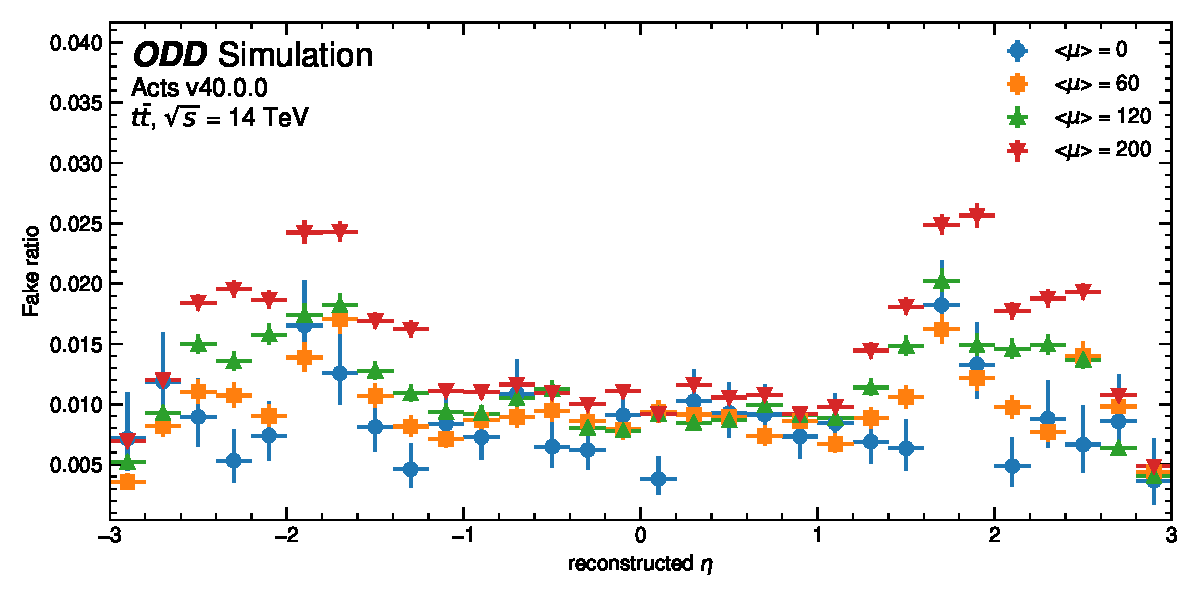
\includegraphics[width=1.0\textwidth]{parts/3_performance/11_odd-performance/figures/finding_fake_ttbar.pdf}
    \caption{Track fake ratio as a function of reconstructed $\eta$ for \ttbar events with different pileup $\langle \mu \rangle$.}
    \label{fig:perf/odd/finding-fake-ttbar}
\end{figure}

Figure \ref{fig:perf/odd/finding-fake-ttbar} shows the track fake ratio for \ttbar events with different pileup $\langle \mu \rangle$ as a function of reconstructed $\eta$. The fake ratio is defined as the number of reconstructed tracks that are not matched to a single truth particle divided by the number of reconstructed tracks. The observed fake ratio is below 2.5\% over the entire $\eta$ range and increases with increasing pilup. Compared to the seeding fake ratio in Figure \ref{fig:perf/odd/seeding-fake-ttbar}, the track fake ratio is significantly lower. This is expected, as the track finding algorithm will try to find all compatible measurements and requires at least 6 for the track to be selected. The triplet seeding depends on only 3 measurements and is therefore more likely to produce fake seeds. The remaining fake tracks will be handled by the ambiguity resolution algorithm, later in the reconstruction chain.

\begin{figure}[h!]
    \centering
    
\includegraphics[width=1.0\textwidth]{parts/3_performance/11_odd-performance/figures/fitting_resolution_d0_vs_eta_mu.pdf}
    \caption{Track resolution of $d_0$ as a function of true $\eta$ for single $\mu$ with $p_T = 1,10,100$ GeV.}
    \label{fig:perf/odd/fitting-resolution-d0-eta-mu}
\end{figure}

Figure \ref{fig:perf/odd/fitting-resolution-d0-eta-mu} shows the resolution of the transverse impact parameter $d_0$ as a function of true $\eta$ for single $\mu$ with $p_T = 1,10,100$ GeV. The resolution is defined as the width of the residual distribution. The residual is defined as the difference between the fitted and simulated truth value $(x^\text{reco} - x^\text{true})$. The resolution is determined by the spatial resolution of the innermost layers, the amount of material travered by the particle, and its momentum. For high momentum paritcles the resolution converges to the intrinsic resolution of the detector, determined by the spatial resolution of the innermost layer.

\begin{figure}[h!]
    \centering
    
\includegraphics[width=1.0\textwidth]{parts/3_performance/11_odd-performance/figures/fitting_resolution_z0_vs_pt_mixed.pdf}
    \caption{Track resolution of $z_0$ as a function of true $p_T$ for single $\mu$, $\pi$, and $e$.}
    \label{fig:perf/odd/fitting-resolution-z0-pt-mixed}
\end{figure}

Figure \ref{fig:perf/odd/fitting-resolution-z0-pt-mixed} shows the resolution of the longitudinal impact parameter $z_0$ as a function of true $p_T$ for single $\mu$, $\pi$, and $e$. The observed resolution is similar for all three particle types across the entire $p_T$ range. At high momentum the resolution converges to the intrinsic resolution of the detector.

\begin{figure}[h!]
    \centering
    
\includegraphics[width=1.0\textwidth]{parts/3_performance/11_odd-performance/figures/fitting_pullmean_vs_eta_mu.pdf}
    \caption{Pull mean of all fitted track parameters at the interaction point as a function of true $\eta$ for single $\mu$ with $p_T = 1,10,100$ GeV.}
    \label{fig:perf/odd/fitting-pullmean-eta-mu}
\end{figure}

Figure \ref{fig:perf/odd/fitting-pullmean-eta-mu} shows the mean of the pull distribution of all fitted track parameters at the interaction point as a function of true $\eta$ for single $\mu$ with $p_T = 1,10,100$ GeV. The pull is defined as the residual divided by the estimated uncertainty of the fitted parameter $(\frac{x^\text{reco} - x^\text{true}}{\sigma_x^\text{reco}})$. The mean of the pull distribution should be 0 for an unbiased parameter estimator. The observed pull mean is close to 0 for all three $p_T$ values. For 100 GeV the pull mean depends on $\eta$ in the non-bending plane $z_0$ and $\theta$.

\begin{figure}[h!]
    \centering
    
\includegraphics[width=1.0\textwidth]{parts/3_performance/11_odd-performance/figures/fitting_pullwidth_vs_eta_mu.pdf}
    \caption{Pull width of all fitted track parameters at the interaction point as a function of true $\eta$ for single $\mu$ with $p_T = 1,10,100$ GeV.}
    \label{fig:perf/odd/fitting-pullwidth-eta-mu}
\end{figure}

Figure \ref{fig:perf/odd/fitting-pullwidth-eta-mu} shows the width of the pull distribution of all fitted track parameters at the interaction point as a function of true $\eta$ for single $\mu$ with $p_T = 1,10,100$ GeV. The width of the pull distribution should be 1 for an unbiased error estimator. The observed pull width is within 5\% to its optimal in the barrel region $|\eta| < 1.0$ for all three $p_T$ values and deviates further outwards with up to 20\%. For 1 and 10 GeV the pull width is generally higher than 1, while for 100 GeV it is lower than 1. This suggests suboptimal material handling or improper scaling of the initial covariance.

\section{Ambiguity resolution performance}

After track finding, the ambiguity resolution algorithm is used to remove duplicate and fake tracks. Generally, it can also be used to resolve cluster ambiguities, when multiple tracks use the same measurement. However, this is not yet implemented in Acts and not part of this study.

The used ambiguity resolution algorithm is based on a greedy approach, where the track with the most shared and fewest measurements is removed first. A detailed description of the algorithm and its implementation is provided in Section \ref{sec:dev/general/greedy-ambiguity-resolution}. The performance of the ambiguity resolution algorithm can be evaluated using the same metrics as for the track finding: efficiency, duplication, and fake ratio.

\begin{figure}[h!]
    \centering
    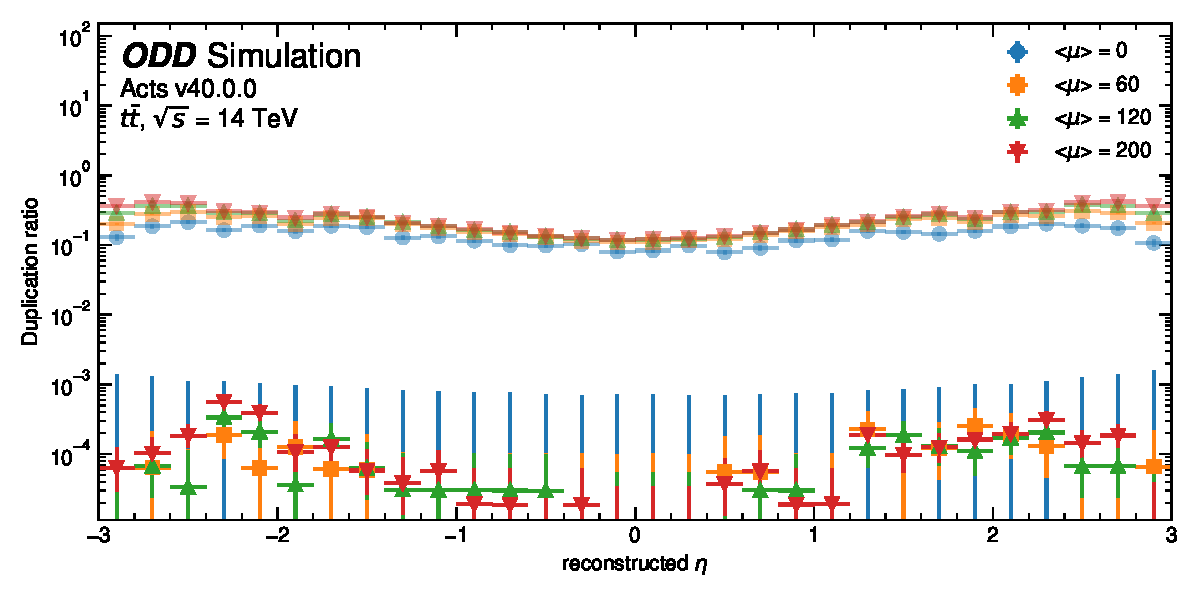
\includegraphics[width=1.0\textwidth]{parts/3_performance/11_odd-performance/figures/ambi_duplication_ttbar.pdf}
    \caption{Track duplication ratio as a function of true $\eta$ for \ttbar events with different pileup $\langle \mu \rangle$. The transparent markers on the top show the track duplication before ambiguity resolution.}
    \label{fig:perf/odd/ambi-duplication-ttbar}
\end{figure}

Figure \ref{fig:perf/odd/ambi-duplication-ttbar} shows the track duplication ratio for \ttbar events with different pileup $\langle \mu \rangle$ as a function of true $\eta$. The transparent markers on the top show the track duplication before ambiguity resolution. The observed duplication drops effectively to 0 in the barrel region $|\eta| < 1$. Outside the barrel, the duplication ratio is about $10^{-4}$.

\section{Track refitting performance}

After track ambiguities are resolved, the tracks are refitted using a Kalman filter. In this study, this is done for demonstraction and validation purposes. In a real experiment, this can be a crucial step to improve the track parameter resolution given more information from other subsystems of the detector, like electron refitting using a Guassian Sum Filter (GSF) after a cluster was found in the electromagnetic calorimeter. A refitting algorithm makes use of the already identified measurements and refined initial parameters from the finding step.

No significant changes in the resolutions and pull means are observed after refitting.

\begin{figure}[h!]
    \centering
    
\includegraphics[width=1.0\textwidth]{parts/3_performance/11_odd-performance/figures/refit_pullwidth_vs_eta_mu.pdf}
    \caption{Pull width of all refitted track parameters at the interaction point as a function of true $\eta$ for single $\mu$ with $p_T = 1,10,100$ GeV.}
    \label{fig:perf/odd/refit-pullwidth-eta-mu}
\end{figure}

Figure \ref{fig:perf/odd/refit-pullwidth-eta-mu} shows the pull width of all refitted track parameters at the interaction point as a function of true $\eta$ for single $\mu$ with $p_T = 1,10,100$ GeV. Compared to the pull widths after finding in Figure \ref{fig:perf/odd/fitting-pullwidth-eta-mu}, the ones after refitting are generally wider than 1. Since the fitter is effectively the same, this suggests that the initial parameters and their covariance are not optimal before track finding.

\section{Primary vertexing performance}

After tracks have been found, ambiguities have been resolved, and the tracks are properly fitted, the primary vertexing algorithm is used to find the primary interactions in the event. For this purpose the Adaptive Multi Vertex Finder (AMVF) is used. This algorithm is specifically desined for high pileup scenarios and allows tracks to be assigned to multiple vertices. The performance of a vertexing algorithm can be quantified by its efficiency in finding vertices, the purity of the reconstructed vertices, and the resolution and pulls of the reconstructed positions. A reconstructed vertex can be built from tracks that are associated to different true interactions. Similarly, tracks from one true interaction can be reconstructed as multiple vertices. Depending on the composition ratios, such a reconstructed vertex may be classified as \textit{merged}. Similarly, depending on the composition ratios, both vertices may be classified as \textit{split}. Otherwise the vertex is classified as \textit{clean}.

This study uses the \texttt{TruthVertexSeeder} for the AMVF. It uses truth information about the vertex positions to create seeds for the finding step and supports time information. Even though the \texttt{AdaptiveGridDensityVertexFinder} has beed adopted to use time information during the work on this thesis, it is not yet fully validated. For this reason and the time dimension support, the \texttt{TruthVertexSeeder} was choosen for this study.

\begin{figure}[h!]
    \centering
    
\includegraphics[width=1.0\textwidth]{parts/3_performance/11_odd-performance/figures/vertex_efficiency.pdf}
    \caption{Technical clean vertex efficiency as a function of pileup $\langle \mu \rangle$ for \ttbar events with and without using the time dimension.}
    \label{fig:perf/odd/vertex-efficiency}
\end{figure}

Figure \ref{fig:perf/odd/vertex-efficiency} shows the technical clean vertex efficiency as a function of pileup $\langle \mu \rangle$ for \ttbar events with and without using the time dimension. With increasing pileup, the gap between efficiency with and without time dimension increases. This suggests that the time dimension is beneficial for the vertexing algorithm, as it allows to better separate vertices. The clean vertex efficiency is about 60\% higher for $\langle \mu \rangle=200$ with time than without. The decreasing efficiency with increasing pileup is due to vertex merging.

\begin{figure}[h!]
    \centering
    
\includegraphics[width=1.0\textwidth]{parts/3_performance/11_odd-performance/figures/vertex_contamination.pdf}
    \caption{Hard-scatter vertex contamination distribution with different pileup $\langle \mu \rangle$ for \ttbar events with and without time. Horizontal lines show maximum, mean, median, and minimum values.}
    \label{fig:perf/odd/vertex-contamination}
\end{figure}

Figure \ref{fig:perf/odd/vertex-contamination} shows the hard-scatter vertex contamination distribution with different pileup $\langle \mu \rangle$ for \ttbar events with and without time. The contamination is defined as the sum of track weight that is not associated to the true interaction divided by the total track weight on the reconstructed vertex. The observed contamination is strictly higher without using the time dimension. This suggests that the time dimension is beneficial for rejecting tracks from pileup interactions.

\begin{figure}[h!]
    \centering
    
\includegraphics[width=1.0\textwidth]{parts/3_performance/11_odd-performance/figures/vertex_resolution.pdf}
    \caption{Hard-scatter vertex resolutions for \ttbar events.}
    \label{fig:perf/odd/vertex-resolution}
\end{figure}

Figure \ref{fig:perf/odd/vertex-resolution} shows the residual distribution of the hard-scatter vertex for \ttbar events. The observed residual distribution centers at 0 for the spatial dimensions and fits well to a gaussian distribution. The $t$ residuals show a bias which is due to the pion particle hypothesis during reconstruction. This is due to particles with significantly different masses from pions, like protons, since they produce biased time of flights. The resolution scale is smaller compared to the track ones, since the vertex fitter will combine the information from all tracks.

\begin{figure}[h!]
    \centering
    
\includegraphics[width=1.0\textwidth]{parts/3_performance/11_odd-performance/figures/vertex_pull.pdf}
    \caption{Hard-scatter vertex pulls for \ttbar events.}
    \label{fig:perf/odd/vertex-pull}
\end{figure}

Figure \ref{fig:perf/odd/vertex-pull} shows pull distribution for the hard-scatter vertex for \ttbar events. The observed pull means are close to 0 for the spatial dimensions. For $t$ we observe the same bias as with the residuals in Figure \ref{fig:perf/odd/vertex-resolution}. The observed pull widths are too wide for the spatial dimensions which is due to the broad track pull widths.

\section{Computational performance}

Computational performance is an important aspect of a reconstruction chain if resources are limited. The computational performance of the reconstruction chain is evaluated using the relative CPU time spent in the different reconstruction steps. The CPU time is measured for \ttbar events with different pileup scenarios.

\begin{figure}[h!]
    \centering
    
\includegraphics[width=1.0\textwidth]{parts/3_performance/11_odd-performance/figures/cpu_total_ttbar.pdf}
    \caption{Relative CPU time for reconstructing \ttbar events as a function of pileup $\langle \mu \rangle$.}
    \label{fig:perf/odd/cpu-total-ttbar}
\end{figure}

Figure \ref{fig:perf/odd/cpu-total-ttbar} shows the relative CPU time for reconstructing \ttbar events with different pileup $\langle \mu \rangle$. The observed CPU time increases superlinearly with increasing pileup. This is due to the increasing hit combinatorics and its impact on the track seeding and finding.

\begin{figure}[h!]
    \centering
    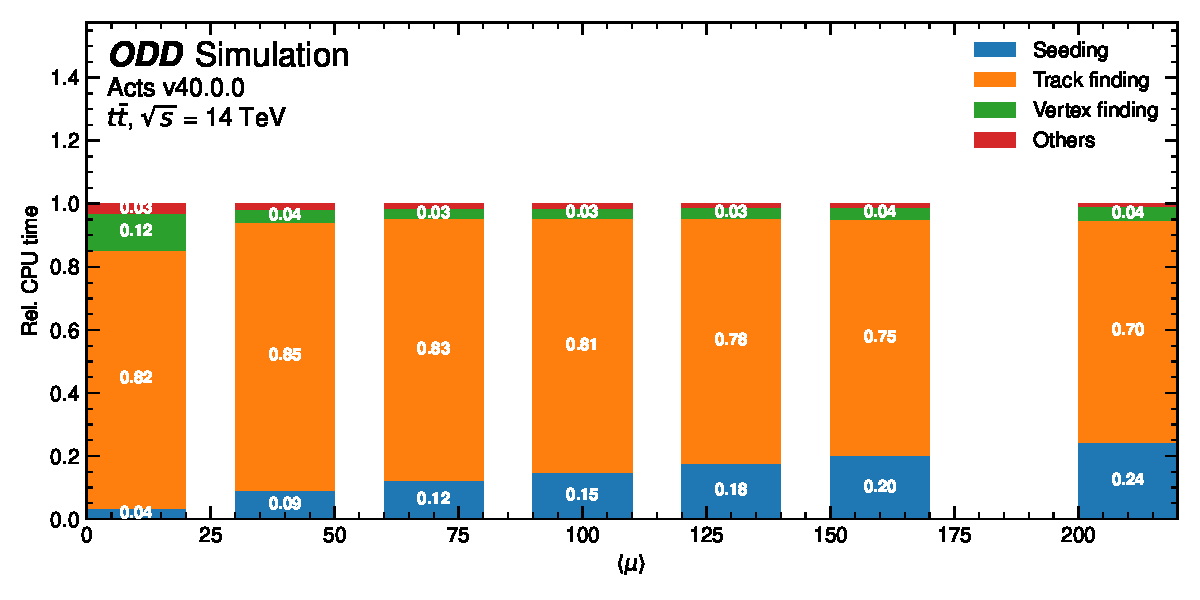
\includegraphics[width=1.0\textwidth]{parts/3_performance/11_odd-performance/figures/cpu_alg_ttbar.pdf}
    \caption{Relative CPU time per algorithm for reconstructing \ttbar events with different pileup $\langle \mu \rangle$.}
    \label{fig:perf/odd/cpu-alg-ttbar}
\end{figure}

Figure \ref{fig:perf/odd/cpu-alg-ttbar} shows the relative CPU time per algorithm for reconstructing \ttbar events with different pileup $\langle \mu \rangle$. The observed CPU time is dominated by the track finding and seeding. Seeding takes an increasing fraction of the CPU time with increasing pileup.

\section{Summary, conclusion and outlook}

The reconstruction performance of the ODD using Acts and its Examples has been evaluated using different event samples. The performance of the individual algorithms has been presented. This includes: seeding, track finding, ambiguity resolution, track refitting, and vertexing. Efficiencies are generally high, with drops in certain detector regions and different particle types. Increasing the performance further, requires optimizing the configuration of the seeding, optimization of the material map, and improving the handling of electrons.

Limitations of this study is the lack of a realistic digitization and the use of a truth-based vertex seeding algorithm. The geometric digitization is not fully validated yet and the performance of the non-truth-based vertex seeder with time information is not fully understood yet. Apart from that, this study used an homogeneous magnetic field and perfect alignment which is not realistic for a real experiment. Future studies can build on this work and include these aspects.
